\chapter{Impulse response and the transfer function}\label{chap:impulseresponse}

In this lab you will be examining the impulse response and the transfer
function of the motor, and the relationship between the two.  Throughout this
lab we will be using the open-loop motor scheme, as depicted in
Figure~\ref{fig:openLoop3}\@,
\begin{figure}[htbp]
\centering
\begin{picture}(200,50)
\put(0,22){$u(t)$}
\put(20,25){\vector(1,0){30}}
\put(55,5){\framebox(105,40)
{\large\((\frac{d^2\theta}{dt^2}+\frac{1}{\tau}\frac{d\theta}{dt})=k_Eu\)}}
\put(165,25){\vector(1,0){30}}
\put(196,22){\(\theta(t)\)}
\end{picture}
\caption{Open-loop motor schematic}\label{fig:openLoop3}
\end{figure}%
but we will be using a constant DC voltage. We will use \textsf{Simulink} to
simulate and implement the system.

\section{Prelab}

The impulse response can be loosely defined as the response of the system to
a ``jolt'' input.  While it is physically impossible to achieve a true
impulse, it is still interesting to study because it reveals much about the
properties of the dynamic system.  Material on impulse response can be found
in Sections 2.4 and 3.5 of the course notes.
 
To make sure that you have a reasonable understanding of the idea of an
impulse response, describe, in words, what happens when a jolt input (a very
short step response) is applied to the motor when: \begin{enumerate} \item
the output is the motor angle, $\theta$; \item the output is the motor
angular velocity, $\omega$. \end{enumerate}

Accompany each with a rough sketch.  You do not have to actually compute
anything, just use your intuition.

\section{Procedure}

\subsection{Impulse Response}\label{cha:impulseRes}

\begin{enumerate}
\item For the open-loop scheme, write out the state equation:
\begin{equation*}
\dot{\vect{x}}=\mat{A}\vect{x}+\vect{b}u,
\end{equation*}
identifying $\vect{x}$\@, $u$\@, $\mat{A}$\@, and $\vect{b}$\@.

\item Determine the output equation:
\begin{equation}
y=\vect{c}^{t}\vect{x}+\mat{D}u,
\end{equation}
identifying $\vect{c}$ and $\mat{D}$ when
\begin{itemize}
\item the output is motor angle, $\theta$\@, and
\item the output is the motor angular velocity, $\omega$.
\end{itemize}

\item Prepare the \textsf{Simulink} model shown in Figure~\ref{fig:model3}.
\begin{figure}[htbp]
\centering
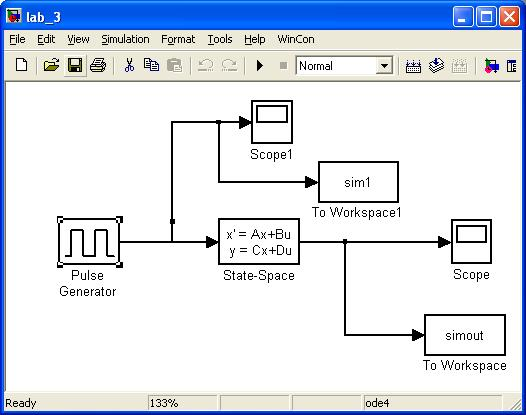
\includegraphics[width=0.6\hsize]{pix/impulseResponseModel.jpg}
\caption{\textsf{Simulink} model for Lab~\ref{chap:impulseresponse}}\label{fig:model3}
\end{figure}%

\item As in Lab~\ref{chap:controlandobserve}\@, enter the motor state
equation using the values of $k_{E}$ and $\tau$ that were estimated in
Lab~\ref{chap:intro} (make sure that you specify the appropriate output).
Double-click on the \verb|Pulse Generator| icon and enter the information as
shown in Figure~\ref{fig:pulseConfig}\@.
\begin{figure}[htbp]
\centering
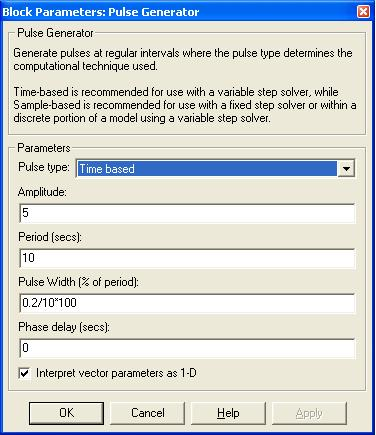
\includegraphics[width=0.6\hsize]{pix/impulseResponsePulseConfig.jpg}
\caption{\texttt{Pulse Generator} configuration for
Lab~\ref{chap:impulseresponse}}\label{fig:pulseConfig}
\end{figure}%
The \verb|Pulse Generator| introduces the impulse function
\begin{equation*}
u_{\epsilon}(t)=\begin{cases}\frac{1}{\epsilon},&
t\leq\epsilon,\\0,&\textrm{otherwise}.\end{cases}
\end{equation*}
every ten seconds.

Recall that the impulse function is defined as
$\lim_{\epsilon\rightarrow0}{u_{\epsilon}}$ (the limit being\ldots er\ldots
in the space of distributions).  Clearly, this is physically impossible to
achieve, but we will approximate as best we can.  The highest voltage that
can be provided by the power supply is 5 volts, so $\epsilon = \frac{1}{5}$
is the lower limit for our system. Pulse width is calculated using the
following formula:
\begin{equation*}
\textrm{Pulse\;Width} = \frac{\frac{1}{\epsilon}}{\textrm{period}}100
\end{equation*}

\item Run the \textsf{Simulink} model. Define the initial conditions to be
zero.  The final time is set to 10 by default.  You may change it by opening
the window
\begin{center}
\verb|Simulation|$\rightarrow$\verb|Configuration Parameters|
\end{center}
and entering the required time in the \verb|Stop time| box.  Start with
$\epsilon=2$ and reduce the value of $\epsilon$ until you see no further
change in the process response.

\item Plot the impulse response for each output described above, using an
appropriate title for each.

\item You will now introduce an impulse into the real system by providing a
``jolt'' by hand. This can be done by tapping the gear.  Prepare the
\textsf{Simulink} model shown in Figure~\ref{fig:model3a}.
\begin{figure}[htbp]
\centering
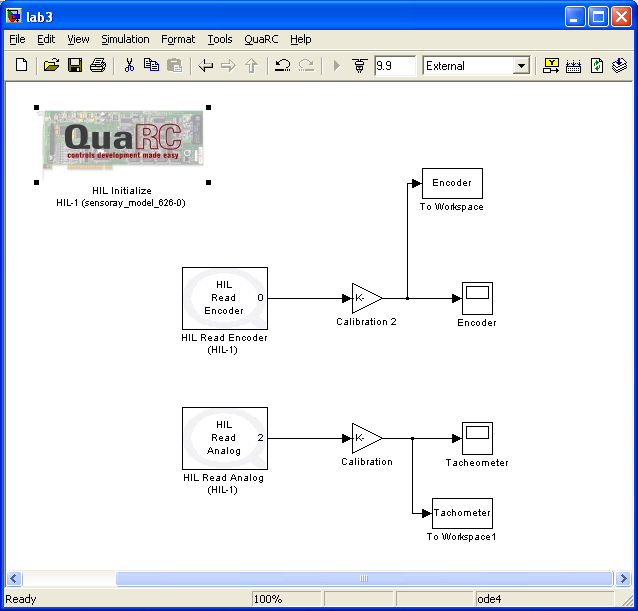
\includegraphics[width=0.6\hsize]{pix/lab3a.jpg}
\caption{Another \textsf{Simulink} model for Lab~\ref{chap:impulseresponse}}\label{fig:model3a}
\end{figure}%
Note that there is no \verb|Write Analog| block required in this case since you are providing the input action.  Using \textsf{Simulink}\@, build the model. Under the Simulation menu, select \verb|Connect to Target|. Then choose \verb|Start Real Time Code|.  Quickly give the motor a ``jolt'' by giving it a quick twist.  Clockwise is taken as the positive direction.

The \verb|Read Encoder| and \verb|Read Analog| parameters are the same as in
Lab~\ref{chap:intro}\@.

\item Plot the response of each state variable while adding an appropriate
title to each plot.

\item Comment on the similarities and differences between the impulse
response and the response of the motor to a hand-powered impulse.

\item To obtain a ``better'' impulse, we introduce the \verb|Pulse Generator|
model as shown in Figure~\ref{fig:model3b}\@.
\begin{figure}
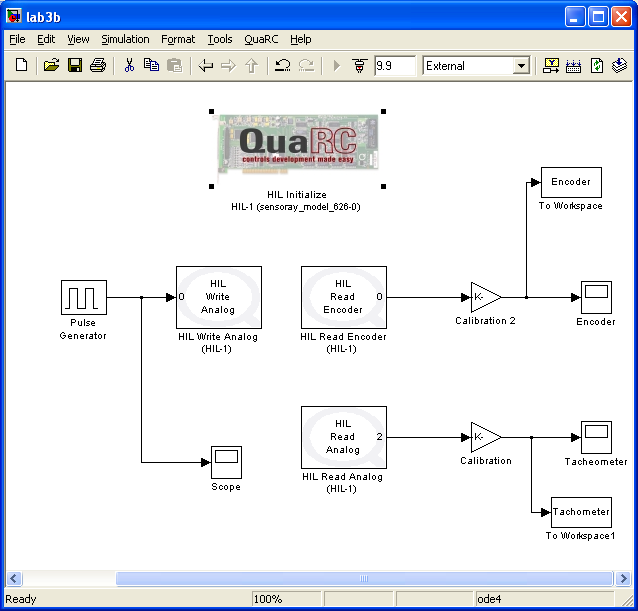
\includegraphics[width=0.9\textwidth]{pix/lab3.PNG} 
\caption{\textsf{Simulink} model for Lab~\ref{chap:impulseresponse}}\label{fig:model3b}
\end{figure}%
Note that the analog output icon has been added since the impulse will be
added automatically in this case.

\item Build and run the model with $\epsilon =1$\@.

\item Run the model again with $\epsilon=\frac{1}{5}$\@.

\item Plot and print the response of the motor angle (encoder input) and the
motor velocity (analog input).  How do these compare with the simulation
impulse response?  With the response due to hand-powered impulse?
\end{enumerate}

\subsection{Transfer Function}

In this part of the lab, you will work in the Laplace transform domain to
analyze this system. Recall that the transfer function $T_{\Sigma}(s)$ is
defined, for example, as the Laplace transform of the impulse response of the
system.
\begin{enumerate}
\item Compute the transfer function from the
standard form, $\dot{\vect{x}}=\mat{A}\vect{x}+\vect{b}u$, $y=\vect{c}^t\vect{x}+\mat{D}u$\@, when
\begin{itemize}
\item the output is the motor angle, $\theta$\@, and
\item the output is the motor angular velocity, $\omega$\@.
\end{itemize}

\item Compute each transfer function again, this time by directly computing
the Laplace transform of the impulse calculated in
Section~\ref{cha:impulseRes}\@.

When you have completed the lab, make sure you save your files in the folder
you created in the Lab~\ref{chap:intro}\@.
\end{enumerate}

%%% Local Variables: 
%%% mode: latex
%%% TeX-master: "lab-manual"
%%% End: 
